%---
\section{Progress and changes to the \DSk\  detector  design}
\label{sec:DSk}

\DSks\ will be located in the Hall-C.  It consists of two detectors: the inner detector and the veto detector, both hosted in a \pDUNE-like cryostat~\cite{Abi:2017wp,Acciarri:2016wz}.   The inner detector is a Liquid Argon Time Projection Chamber (\LArTPC) filled with \UAr.  The veto detector is made of a plastic shell, loaded with Gd, surrounding the inner detector, sandwiched between two active AAr layers.
 \reffig{DSk3D} shows a 3D schematics, with the inner detector placed at the middle position of the veto detector.

\begin{figure}[t!]
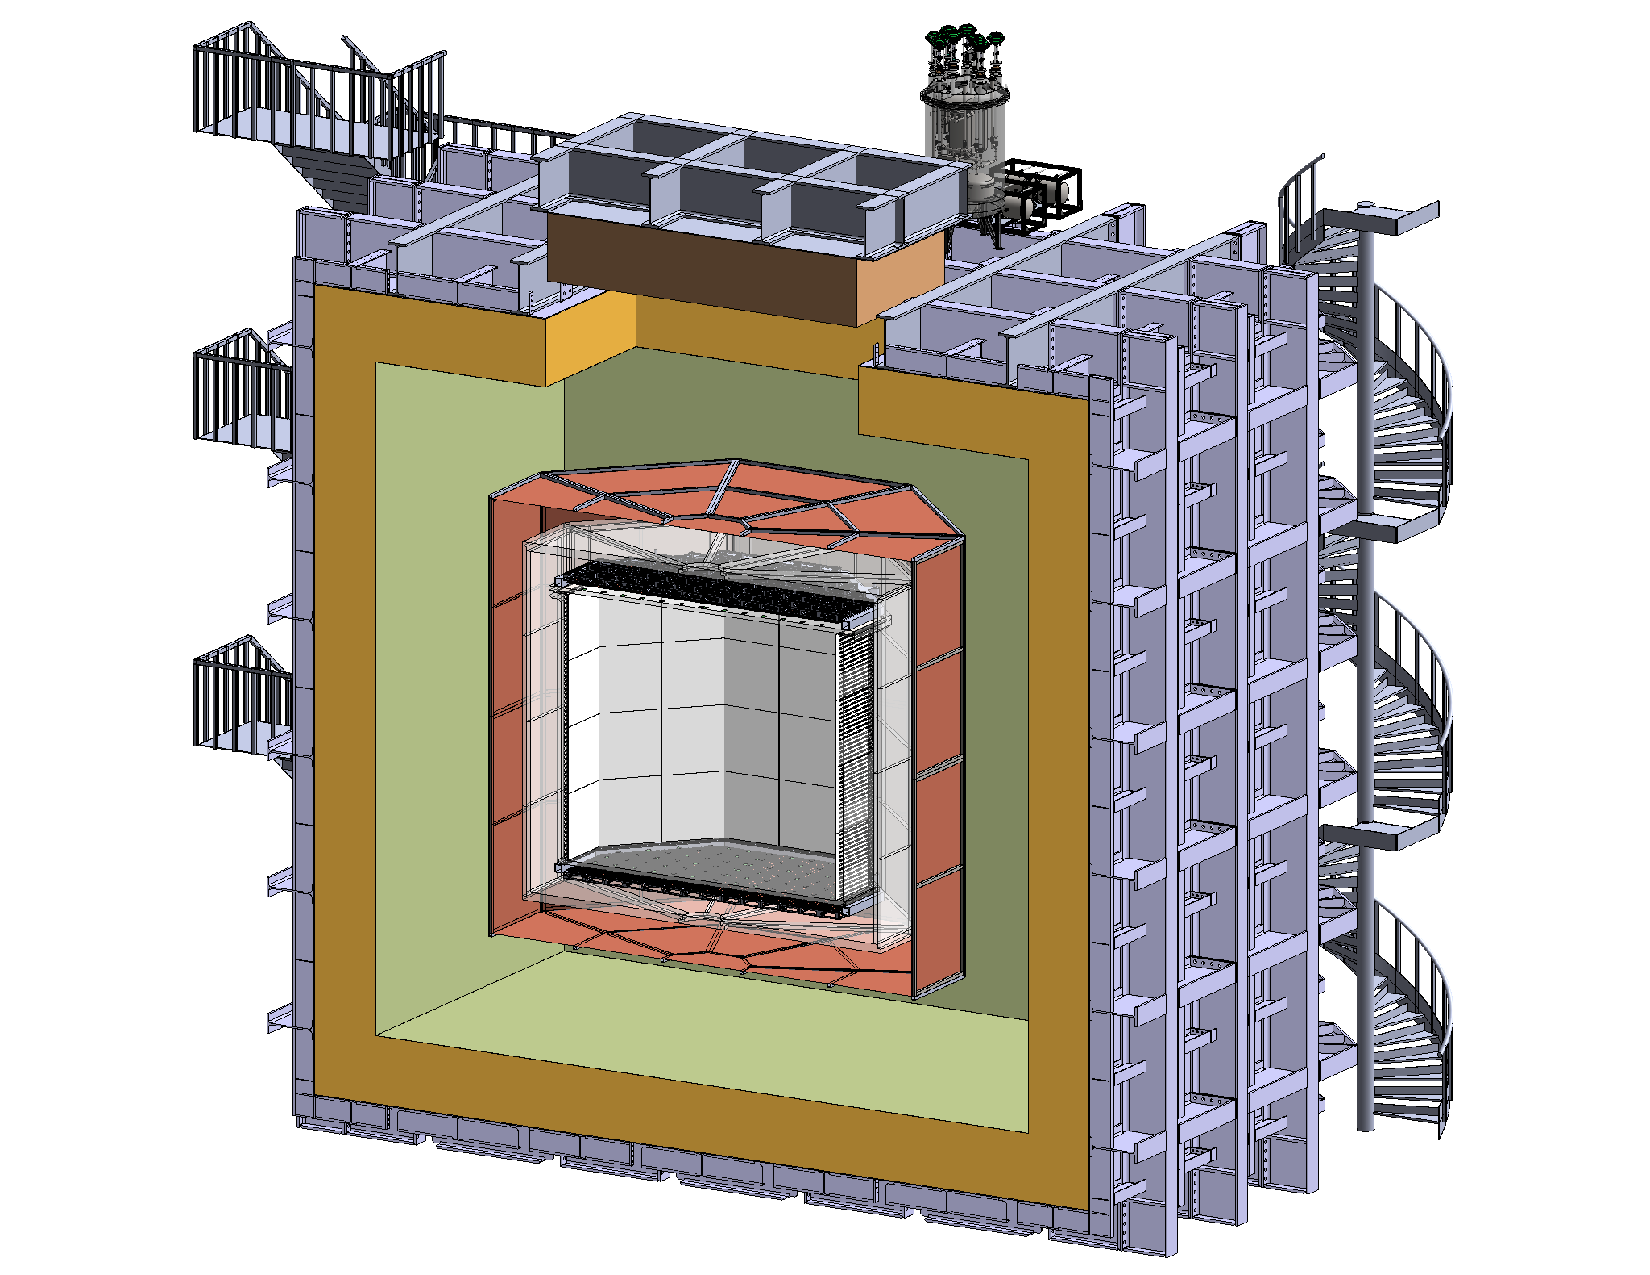
\includegraphics[width=\columnwidth]{Figures/DSk3D.pdf}
\caption{3D schematics of the \DSk\ experiment.  The drawing shows  the PPMA  TPC  filled with UAr, surrounded by the VETO detector made of Gd-loaded  PMMA  shell sandwiched between two AAr active layers (the inner one, named IAB and the outer one, named OAB in the text), all contained in the  \pDUNE-like cryostat. The OAB is optically separated by the AAr in  contact with the cryostat wall by a membrane, whose characteristics are yet to be defined. }
\label{fig:DSk3D}
\end{figure}

The decision to abandon an organic liquid scintillator veto and to host \DSks\ within a \pDUNE-like cryostat was originally motivated by the need of minimizing the environmental impact on underground \LNGS\ operations, but carries significant performance advantages.  Indeed, operating the \TPC\ directly in the  \pDUNE-like cryostat  allows to eliminate the stainless steel (SS) cryostat, the leading contribution to the residual background. We are therefore studying  a new design, with the \TPC, with its \UAr\ fill,  immersed in bath of liquefied \AAr\ at the same temperature and pressure.  This permits to build the \TPC\ of the same ultra-pure poly(methyl methacrylate) (\PMMA) developed for the \DEAP\ experiment, eliminating the need for a dedicated cryostat or \UAr\ containment vessel.  The outer walls of the \TPC\ will sit approximately \SI{2}{\m} away from inner wall of the cryostat.  The \pDUNE-like cryostat will be surrounded by layers of plastic for moderation of cosmogenic and radiogenic neutrons from the rocks surrounding the \LNGS\ Hall~C.